\documentclass{article}
\usepackage[margin=1in]{geometry}
\usepackage{graphicx}
\usepackage{enumitem}
\usepackage[toc,page]{appendix}
\usepackage{amsfonts}
\usepackage{amsmath}
\usepackage{amsthm}
\usepackage{commath}
\usepackage{color}

\title{FLASH Orchestration System Design}

% No automatic indenting
\setlength\parindent{0pt}

% Set spacing between items in itemize/enumerate
\setlist{itemsep=1pt}

\newcommand{\N}                 {{\mathbb N}}
\newcommand{\Z}                 {{\mathbb Z}}
\newcommand{\Q}                 {{\mathbb Q}}
\newcommand{\R}                 {{\mathbb R}}
\newcommand{\C}                 {{\mathbb C}}
\newcommand{\F}                 {{\mathbb F}}

\newcommand{\SetuptimeParam}[1] {\textcolor{red}{#1}}
\newcommand{\RuntimeParam}[1]   {\textcolor{blue}{#1}}
\newcommand{\ComposerKey}[1]    {\textcolor{cyan}{#1}}

\newcommand{\TeamStarting}      {\textsc{TeamStarting}}
\newcommand{\TeamIdle}          {\textsc{TeamIdle}}
\newcommand{\TeamRunningOpen}   {\textsc{TeamRunningOpen}}
\newcommand{\TeamRunningClosed} {\textsc{TeamRunningClosed}}
\newcommand{\TeamRunningNoMoreWork} {\textsc{TeamRunningNoMoreWork}}
\newcommand{\TeamTerminating}   {\textsc{TeamTerminating}}

\newcommand{\ThreadStarting}    {\textsc{ThreadStarting}}
\newcommand{\ThreadIdle}        {\textsc{ThreadIdle}}
\newcommand{\ThreadComputing}   {\textsc{ThreadComputing}}
\newcommand{\ThreadWaiting}     {\textsc{ThreadWaiting}}
\newcommand{\ThreadTerminating} {\textsc{ThreadTerminating}}

\begin{document}

% Setup numbered/referentiable environment for requirements
\theoremstyle{definition} % No italics or spaces
\newtheorem{req}{Req}[section]

\maketitle

\section{Design Summary}

\section{Runtime Requirements}
If a simulation is setup such that no runtime is needed, then the Orchestration
runtime shall not be built into the simulation.  In particular, this means that
there shall be no unnecessary resources allocated nor an extra level of packing
tiles into data packets.  This could allow for basic stub implementations such
as initialization/finalization being called from Driver.\\

At any point in time during the execution of a simulation, there shall be no more
than one instantiation of the runtime in operation so that design complexity can
be minimized (\textit{e.g.} resource allocation and management).\\

The runtime shall be built into FLASH5 as a new unit and the unit shall allow
for different implementations of the unit.  Some examples of different
implementations will be
\begin{itemize}
\item{low-level (\textit{e.g.} CUDA Fortran) \textit{vs.} high-level
(\textit{e.g.} OpenMP) and}
\item{general (\textit{e.g.} CUDA Fortran) \textit{vs.}} platform-specific
(\textit{e.g.} CUDA Fortran optimized for Summit).
\end{itemize}

The interface of the runtime unit will allow for running a bundle of auxiliary
tasks and a bundle of work tasks.  \textcolor{red}{Should we allow for bundles
that are a mixture of auxiliary and work tasks?}\\

The interface of the runtime shall be designed such  that when a new type of
device is introduced in platform nodes, the routines for starting a runtime
execution can be extended trivially\footnote{Ideally by adding new function
pointers to the parameter list of these routines.} for including the running of
tasks on these devices.  If the nodes allow for running concurrently tasks on
this device while running code on the host or on other devices, then the updated
interface shall allow for this.\\

\textcolor{red}{Put in information regarding runtime parameters needed by
runtime.  Does this include runtime parameters that depend upon how task were
bundled/scheduled?}\\

\textcolor{red}{Do we allow for specifying to the runtime which data should
remain where?}\\

At instantiation, the runtime shall instantiate a given number, $N$, of distinct
thread teams and each thread team shall be allowed to simultaneously use
at most a given number, $M$, of threads.  \textcolor{red}{It remains to be seen
if the threads should be created at instantiation and persist throughout the
simulation or if they should be created each time the runtime executes a task
bundle.  The former would be more runtime efficient, but permanently consume
more memory in the form of thread stacks, etc. and increase the burden on the
OS.}\\

Thread teams shall
\begin{enumerate}
\item{be created and run in the host CPU,}
\item{be associated with a single MPI rank, and}
\item{expose the same interface to client code.}
\end{enumerate}

A thread team shall be used by client code to apply a single, given
computational task to all blocks managed by the team's associated MPI rank in
each runtime execution cycle.  Note that the computational task can be different
with each cycle.  \textcolor{red}{Should we allow for dividing the load of blocks
between two or more thread teams?  For example, if the task bundle
has effectively just one task, we could have half the blocks run on the CPU and
the other half on the GPU.  Should we allow for the possiblity of a thread that
determines dynamically to which thread team it should give the next block?  This
could be a way of making full use of HW.  This implies that all thread teams in
the selection pool could also be work publishers to the same thread team that
applies a follow-up task to all blocks.}\\

Thread teams shall not need to know nor be informed of which device will carry
out the computation associated with a given computational task.  Rather the
given computational task shall know where its block data resides in different
memory and the task shall be written so that it can carry out its computations
on the devices assigned to it.  This can include running code on the host CPU
with the given team thread or using the team thread to launch computations on
accelerator devices.\\

A thread team shall execute at most one task at a time so that it is easier to
determine independence of tasks and teams.  For each task execution the client
code shall inform the thread team what task shall be executed and how many
threads in the team should be activated immediately to start work on the task.\\

The thread team interface shall allow for client code to assign more units of
work to a thread team and this shall only be allowed if the thread team is in the
\TeamIdle or \TeamRunningOpen states.  This requirement is consistent with
requirement XXX in that and is \emph{not} inconsistent with requirement YYY as
this requirement relates to what happens once the team is already in the
\TeamIdle state.  Each execution cycle for a given thread team begins
\begin{enumerate}
\item{with the thread team in \TeamIdle if it is the case that client code has
chosen to already give units of work to the thread team or}
\item{when client code gives the team a computational task and triggers the
team's state to \TeamRunningOpen otherwise.}
\end{enumerate}

Client code shall trigger \textit{via} the runtime interface a single runtime
execution cycle that consists of executing potentially many distinct tasks on
multiple different target devices.  Based on the number of tasks in the cycle's
task bundle, the runtime will assemble the appropriate topology of thread teams.
The runtime shall trigger an error if the number of tasks in the bundle is more
than the number of thread teams created by the runtime.\\

The lead thread that is used to trigger/schedule a runtime execution cycle shall
gather tiles using the Grid unit's tile iterator (or asycnrhonous tile
iterator), form these into the appropriate units of work, and give the units of
work to the appropriate thread teams.\\

A thread team may be configured to push units of work, to which it has already
applied its task, to other thread teams.  The team that pushes units of work is
therefore a \textbf{work publisher} and the teams to which the units of work are
given are \textbf{work subscribers}.  A thread team shall not be allowed to push
work to itself.  It shall be possible for a single thread team to be a work
subscriber for two distinct work publishers\footnote{Split the load of blocks
between a thread team dedicated for FPGAs and a second team for GPUs.  We could
have each team run the same task on its subset of blocks and then pipe the
results into a single work subscriber that runs a quick, independent follow-up
task on the CPU.}\\

Each thread team may be configured as a \textbf{thread publisher} and as a
\textbf{thread subscriber}.  A thread publisher shall have at most one thread
subscriber and there shall be no limit to the number of thread publishers that a
thread subscriber can have.  When a thread in a thread publisher team
transitions to \ThreadIdle, the thread publisher shall inform its
single\footnote{This requirement is related to load balancing and in this sense,
we cannot activate a thread in each of several thread teams because one thread
has transitioned to \ThreadIdle.  We could build in a round-robin communication
scheme but choose not to in the name of simplicity.} subscriber that the
subscriber can now activate another thread in its team.  The requirements allow
for a single thread team being both a subscriber and a publisher.  A thread team
shall not be alloed to push a thread to itself.\\

If a thread subscriber is informed that it may activate another thread in its
team but there are no more threads in the team in the \TeamIdle state, then the
subscriber team shall emit an error.  Therefore, it is the client code's
responsibility to ensure that the number of threads in a thread subscriber team
is less than or equal to the sum total of threads that the team starts with and
the number of threads that can be triggered.  Note that multiple thread teams
can be connected in chains and a single thread team could be a subscriber to
many chains.  Therefore, the task of determining the maximum number of threads
in a team is important and can be challengning.\\

TODO: Add info how pub/sub links are made and when they can be made/unmade.\\

TODO: Need to specify requirements for unit of work translation.\\

\section{Runtime Technical Specifications \& Design}
%What classes of scalar values do we have in the physics units?  For instance are
%there scalars that are constant for the duration of the simulation?  Constant
%for the duration of an iteration?  Constants that are changed by auxiliary
%tasks?  Constants that are updated by work tasks?  For the first two, we can set
%up mirrors of the variable between host and devices.  Those that are changed by
%auxiliary tasks can also be mirrored by running the task concurrently in both
%the CPU and the GPU.  What about the others?  Do we send those in the data
%packets so that the CPU and GPUs can force the mirroring somehow?  Do we just
%hand these over the managed memory and hope that everything goes well?  Do we
%hand these over to managed memory but ask the task composer to touch the scalars
%on the appropriate device before each runtime call (these are blocking)?\\

The runtime is fundamentally a event-driven software and as such the design has
been specified as a finite state machine.  However, the behavior in a given
state cannot be specified solely on the basis of a single qualitative state
variable.  Rather, the behavior will depend on a qualitative state variable,
which is called the mode, as well as the quantitative internal state variables
$N_i, N_w, N_c, N_t, N_Q$ that respectively keep track of 
\begin{itemize}
\item{the number of idle threads in the team,}
\item{the number of threads that are waiting for work to be added,}
\item{the number of threads executing a computation on a unit of work,}
\item{the number of threads that are terminating, and}
\item{the number of units of work in team's pending work queue.}
\end{itemize}
Note that the definitions of $N_i, N_w, N_c, N_t$ imply that each thread is
always in one and only one state but that this EFSM need not track the actual
state of each thread --- it is only the aggregated thread state information that
is important.  Therefore, the runtime is an extended finite state machine 
\[
M = (Q, X, I, O, s_0, T)
\]
where
\begin{itemize}
\item{$Q$ is the finite set of qualitative modes,}
\item{$X = \set{(N_i, N_w, N_c, N_t, N_Q) \in \N_0^5 | N_i + N_w + N_c + N_t =
N_{max}}$ is the set of internal state variables where $N_{max}$ is the
number of threads in the team,}
\item{$I$ is the set of internel and external events,}
\item{$O$ is the set of outputs,}
\item{$s_0 = (q_0, x_0) \in Q \times X$ is the initial state, and}
\item{$T : Q \times X \times I \to Q \times X \times O$ is the transition
function that is evaluated by the EFSM at each occurrence of an event to
identify the output to be performed as well as the state to transition to.}
\end{itemize}

The set $Q$ contains the modes
\begin{itemize}
\item{\TeamIdle --- all threads idle and no work in the queue}
\item{\TeamRunningOpen --- a task has been given to the team and units of work
on which to execute the task can still be given to the team}
\item{\TeamRunningClosed --- a task being executed but no more units
of work can be given to the team}
\item{\TeamRunningNoMoreWork --- a task is being executed, no more
units of work can be given, and the team has identified that the task has
already been applied to or is currently being applied to all units of work}
\item{\TeamTerminating --- the client has indicated that it no longer needs the team.}
\end{itemize}

The set $I$ of events is the union of events triggered by clients through the
team's interface
\begin{itemize}
\item{\texttt{startTask} --- give the team a task and activate a given number of the
$N_{max}$ idle threads in the team to work on it}
\item{\texttt{increaseThreadCount} --- activate a given number of idle threads in the
team so that they can start working on the task as well}
\item{\texttt{enqueue} --- give the team a unit of work on which to apply its
task}
\item{\texttt{closeTask} --- indicate (without blocking the caller) to the team
that no more units of work will be given for the current task}
\item{\texttt{$\sim$ThreadTeam} --- thread team no longer needed}
\end{itemize}
with the set of events triggered internally
\begin{itemize}
\item{\texttt{activateThread} --- wake an idle thread so that it can participate
in applying a task to given units of work}
\item{\texttt{transitionThread} --- wake a thread that is waiting for work so
that it can evaluate if there is pending work and update its state accordingly}
\item{\texttt{computationFinished} --- a thread finished applying the team's
task to a unit of work and shall evaluate if there is pending work and update
its state accordingly}
\item{\texttt{threadTerminated} --- emitted by a thread to indicate that it has
terminated}
\end{itemize}

The initial state is defined to be
\[
s_0 = \left(q_0, (N_i, N_w, N_c, N_t, N_Q)_0\right) = \left(\TeamIdle, (0, 0, 0, 0, 0)\right).
\]

The set $O$ and the transition function $T$ encapsulate the complexity of the
runtime and are specified in the spreadsheet XXX.  A state diagram for the team
that indicates only states and transitions is shown in
Figure~\ref{fig:TeamStateDiagram}.  A similar state diagram for threads in the
team is shown in Figure~\ref{fig:ThreadStateDiagram}.  These figures are
intended only to aid in understanding the design of the runtime.  The content of
XXX should be understood to be the actual design of the runtime.

\begin{figure}[!ht]
\begin{center}
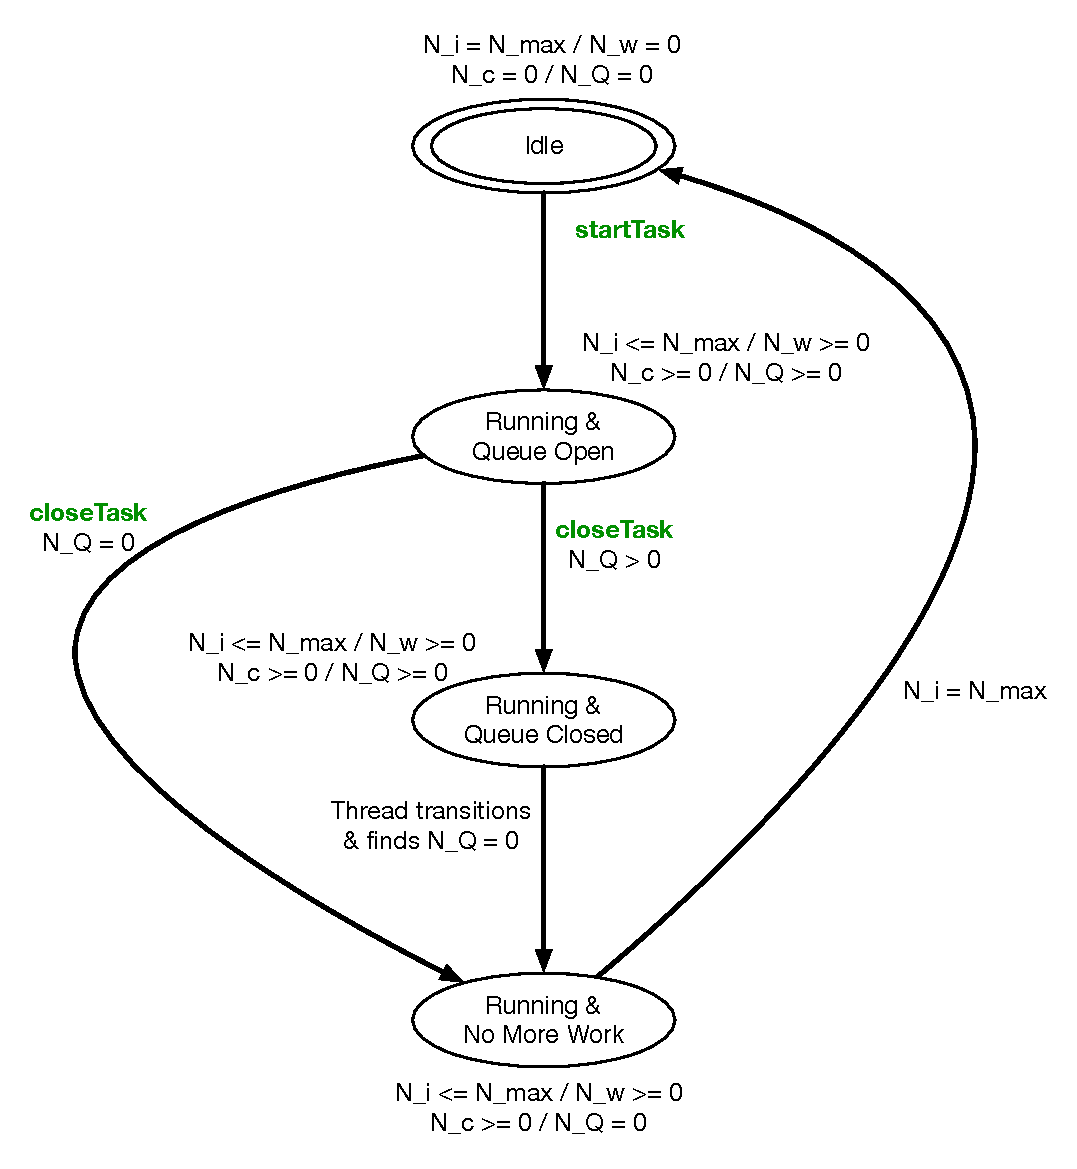
\includegraphics[width=5.0in]{TeamStates.pdf}
\caption[]{}
\label{fig:TeamStateDiagram}
\end{center}
\end{figure}

\begin{figure}[!hp]
\begin{center}
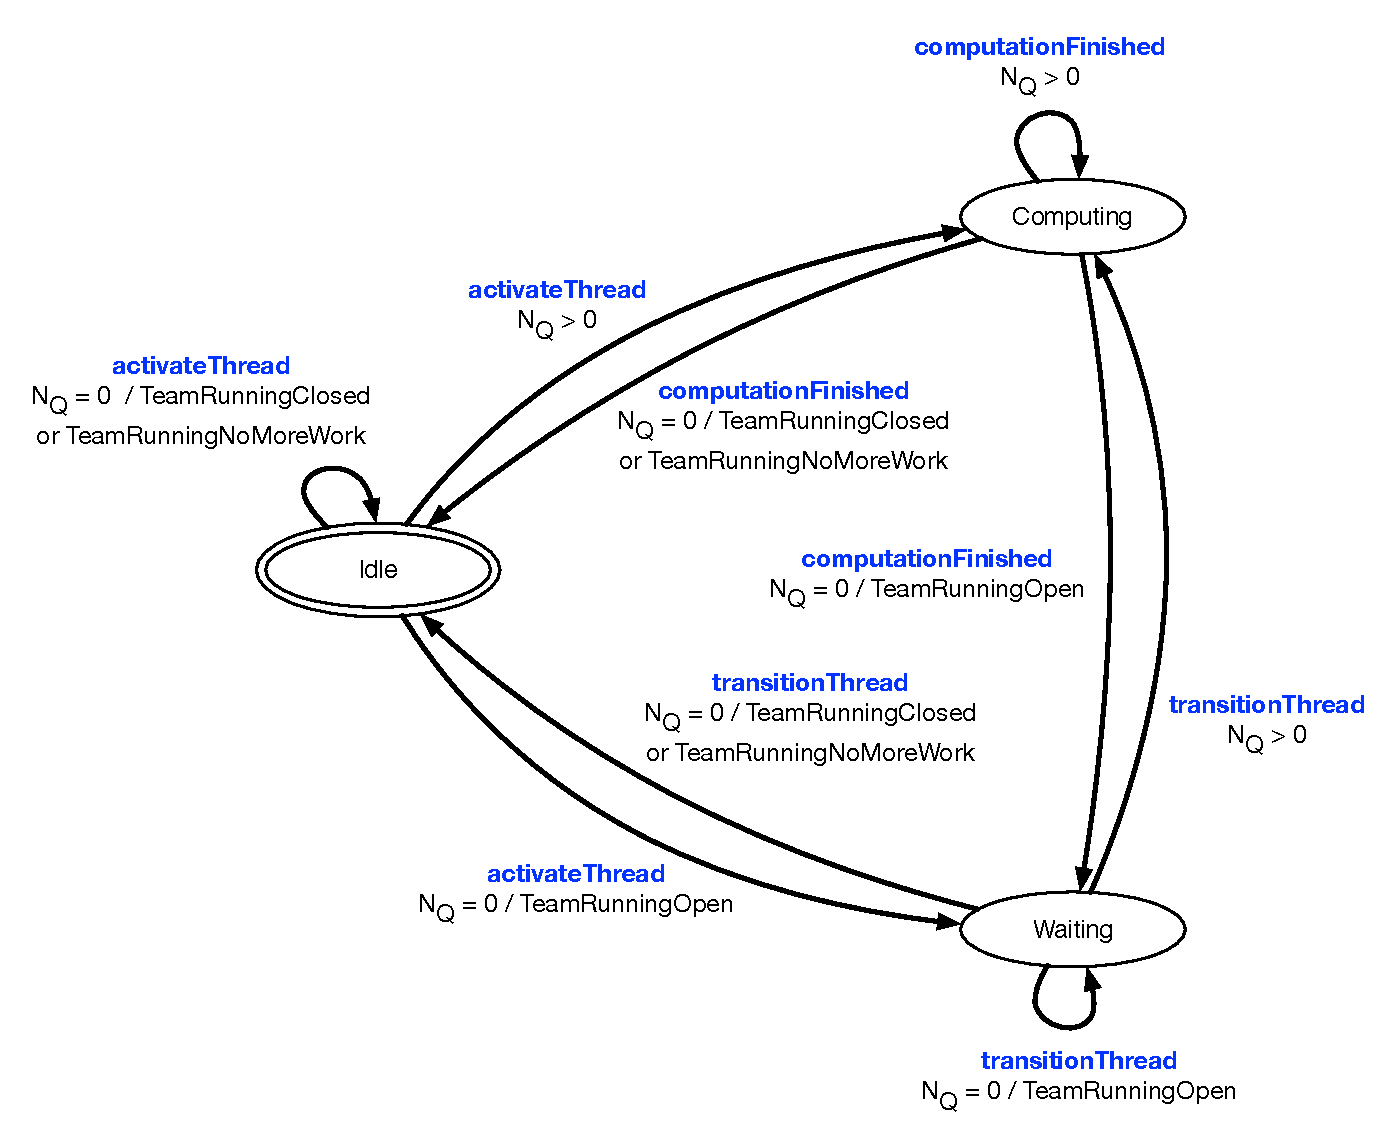
\includegraphics[width=6.5in]{ThreadStatesPersistent.pdf}
\caption[]{}
\label{fig:ThreadStateDiagram}
\end{center}
\end{figure}

\begin{req}
All threads that transition to idle must wait for the \texttt{activateThread}
signal.
\label{req:IdleActivateThread}
\end{req}

\begin{req}
External code can decrease $N_i$ through the \texttt{startTask} and
\texttt{increaseThreadCount} events and the runtime shall be implemented such
that a request to activate $i$ threads results in an error if $i$ exceeds the
number of idle threads that are available for activation.
\end{req}
\textbf{Verification:}\hspace{0.125in}  In the present design, this requirement
is important because the runtime would emit more \texttt{activateThread} signals
than there are threads to receive them.  Because teams allows for thread
publishers/subscribers, undetected signals would amount to a loss of thread
resources at the level of the runtime.  Note that a thread-based implementation
will have a lag between when these events trigger the activation of idle threads
and when these threads are actually activated.  The runtime design therefore
tracks the actual number of idle threads with \texttt{N\_idle\_} = $N_i$ as well
as the number of threads pending activation with \texttt{N\_to\_activate\_}.
When a thread does receive \texttt{activateThread}, it decrements both
\texttt{N\_idle\_} and \texttt{N\_to\_activate\_} and increments the internal
state variable $N_w, N_c$, or $N_t$ corresponding to the thread's next state.
To satisfy the requirement, both events throw an error if $i > $
\texttt{N\_idle\_} - \texttt{N\_to\_activate\_}.

\begin{req}
\label{req:Runtime_OneWait}
For each task execution, a team shall allow for only one thread to wait on the
termination of the task.
\end{req}
\textbf{Verification:}\hspace{0.125in}  Implemented a flag
\texttt{isWaitBlocking\_} to track if a thread has already called \texttt{wait}.

\begin{req}
To maintain a simple design, client code shall only be allowed to attach and
detach thread subscribers when the team is in the {\TeamIdle} mode.  The same
requirement applies for work subscribers.
\end{req}
\textbf{Verification:}\hspace{0.125in}

\subsection{{\TeamIdle} State}

\begin{req}
\label{req:Idle_NoEnqueue}
While the runtime could allow clients to give units of work to a team with the
understanding that the work would be for the next task to be given to the team,
there is no known use case for which this is necessary.  Therefore, to simplify
the design, client code shall not be allowed to give a team a unit of work if
the team is in the mode \TeamIdle.  
\end{req}
\textbf{Verification:}\hspace{0.125in}  The \texttt{enqueue} method throws an
error if called in this mode.  There is no other means to add work.\\ 

\begin{req}
In the {\TeamIdle} mode, the queue shall always be empty and all threads in the
team in the idle state.  This implies that no thread can be in the Waiting,
Computing, or Terminating states and that all threads are therefore by
Req~\ref{req:IdleActivateThread} are waiting to receive the
\texttt{activateThread} event.
\end{req}
\textbf{Verification:}\hspace{0.125in}  The initial state starts in {\TeamIdle}
but specifies that there is no work in the queue.  Also, all transitions to
{\TeamIdle} can only happen if the queue is empty.  Therefore, the pending work
queue is always empty upon entry to \TeamIdle.  Finally, no work can be added
to the queue in the {\TeamIdle} state by Req~\ref{req:Idle_NoEnqueue}.\\

The initial state specifies that all threads are idle and transitions to
{\TeamIdle} can only happen if the same is true.  Therefore, the claim is true
upon entry to {\TeamIdle} and all threads are waiting for \texttt{activateThread}.
Note that threads can only transition to Terminating in the {\TeamTerminating} 
state.  Also, responses\footnote{These cases are being considered should one of
these events be emitted when the team in not Idle, but is received after
transitioning to Idle.  With the current implementation, since all threads would
be waiting on \texttt{activateThread}, no threads would be waiting for the
latter two events.} to \texttt{activateThread}, \texttt{transitionThread}, and
\texttt{computationFinishes} do not transition the thread state and have the
responding threads wait for \texttt{activateThread}.  Therefore any attempt to
transition a thread terminates with the thread in idle.\\

\begin{req}
Consider a team that is both a thread publisher and subscriber.  It is possible
for the team to finish its work and transition to {\TeamIdle} before its
publisher finishes its work.  Therefore, to avoid loss of thread resources at
the level of the runtime, teams that are thread publishers and that are in
{\TeamIdle} shall forward requests to increase thread count on to their
subscriber.
\end{req}
\textbf{Verification:}\hspace{0.125in}  Implemented directly as stated.

\begin{req}
It is possible that a runtime execution cycle could finish and transition the
team back to {\TeamIdle} before an external thread has the chance to call
\texttt{wait}.  Therefore, the method shall be enabled in {\TeamIdle} and shall
terminate immediately to avoid unnecessary blocking of the calling thread.  Note
that this does allow for client code to superfluously call \texttt{wait} before
the first execution cycle is run and multiple times between cycles, both of
which are logical errors.
\end{req}
\textbf{Verification:}\hspace{0.125in}  Implemented directly as stated and in
accord with Req~\ref{req:Runtime_OneWait}.  


\subsection{{\TeamTerminating} State}
\begin{req}
Client code shall not be able to interact with a thread team that is in the
{\ThreadTerminating} mode and the EFSM terminates automatically as a result of
being transitioned to this mode.
\end{req}
\textbf{Verification:}\hspace{0.125in} The transition to this mode is triggered
by destroying the team object and is therefore handled by the destructor.
Hence, interaction with the object is impossible.

\begin{req}
Upon entry into {\TeamTerminating} and while in this state, the pending work
queue shall always be empty and the number of waiting and computing threads
equal to zero.
\end{req}
\textbf{Verification:}\hspace{0.125in}  These are confirmed in the destructor
upon transitioning to the mode.  Other consistency checks are handled in the
destructor as sanity checks of proper implementation.

\subsection{\TeamRunningOpen}
\begin{req}
Consider the case of two teams, one of which is the work publisher for the
other.  When the publisher team transitions to {\TeamRunningNoMoreWork}, it
calls the subscriber's \texttt{closeTask()} method to inform the subscriber that
it will not be given more work.  This implies that the thread that executes an
execution cycle with the Orchestration Runtime does not know when
\texttt{closeTask()} is called and therefore could call \texttt{wait()} before
this event occurs.  Hence, a thread team in the state {\TeamRunningOpen} shall
allow for a thread to call \texttt{wait()} method.
\end{req}
\textbf{Verification:}\hspace{0.125in}  Implemented directly as stated.

\begin{req}
\end{req}
\textbf{Verification:}\hspace{0.125in}


At any point in time, each thread team shall only exist in one of the states
\begin{enumerate}
\item{\TeamStarting,}
\item{\TeamIdle,}
\item{\TeamRunningOpen,}
\item{\TeamRunningClosed, or}
\item{\TeamTerminating.}
\end{enumerate}

A thread team shall be set into the \TeamStarting state upon creation and the
team's state shall not transition to \TeamStarting from any state. \\

A thread team's state can transition to \TeamIdle only if
\begin{enumerate}
\item{the current state is \TeamStarting or \TeamRunningClosed and}
\item{all threads in the team are created and in the state \ThreadIdle.}
\end{enumerate}
If the current state is \TeamRunningClosed, then the transition to \TeamIdle
shall occur automatically without client code intervention once all threads in
the team have transitioned to the state \ThreadIdle.\\

A thread team state shall transition from \TeamStarting to \TeamIdle
automatically once all requirements for transitioning to \TeamIdle are
satisified.  \textcolor{red}{For the present design, this means that
\TeamStarting is a transitory state and the team can only be in that state
during the construction phase of a thread team.}\\

A thread team's state can be transitioned to \TeamRunningOpen only if
\begin{enumerate}
\item{the current state is \TeamIdle and}
\item{the client code has triggered this \textit{via} the thread team's
interface (\texttt{startTask()}).}
\end{enumerate}

A thread team's state can be transitioned to \TeamRunningClosed only if
\begin{enumerate}
\item{the current state is \TeamRunningOpen and}
\item{the client code has triggered this \textit{via} the thread team's
interface (\texttt{closeTask()}).}
\end{enumerate}

A thread team's state can be transitioned to \TeamTerminating only if the
current state is \TeamIdle, which implies that no thread in the team is working.
In addition, this transition must require that there be no pending work for the
team (\textit{e.g.} no units of work given to the thread team while in the
\TeamIdle state).  \textcolor{red}{As with \TeamStarting, \TeamTerminating is
presently implemented as a transitory state and the transition to this state can
only be triggered by client code destroying the thread team}.\\

The state of a work subscriber shall be transitioned to \TeamRunningClosed only
by its work publisher and only once the work publisher has determined that it
has no more pending work and no more work can be added to its set of pending
work.  \textcolor{red}{How to deal with this if we allow for a subscriber to
have multiple publishers?  Publishers call a routine in subscriber to inform the
subscriber that it can detach and subscriber transitions to closed only once it
is not attached to any subscribers?  This implies pub/sub pattern with two way
knowledge of relationship.}\\

TODO: Add in information about when work can be added.  Add in info about when
Work/Thread subscribers can be added/removed.  Need to account for special cases
of threads being given.\\


At any point in time, each thread in a thread team shall only exist in one of
the states
\begin{enumerate}
\item{\ThreadStarting,}
\item{\ThreadIdle,}
\item{\ThreadComputing,}
\item{\ThreadWaiting, or}
\item{\ThreadTerminating.}
\end{enumerate}

A thread shall be set automatically into the \TeamStarting state by its thread
team upon creation of both the team and the thread itself.  The thread's state
shall not transition to \ThreadStarting from any state. \\

A thread's state can transition to \ThreadIdle only if
\begin{enumerate}
\item{it is presently in any state other than \ThreadTerminating,}
\item{the thread is not presently executing work,}
\item{there is no work pending for the thread's team, and}
\item{there is no possibility of more work being given to the thread's team
during the current execution cycle.}
\end{enumerate}
This requirement and requirement XXX imply that a team cannot transition to the
state \TeamIdle unless there is no more work and no possibility for more work to
be given to the team if the team is executing a task.\\

A thread's state shall only be transitioned to \ThreadTerminating by the
thread's team and this transition shall and shall only occur when the
state of the thread's team is transitioned to \TeamTerminating.\\

A thread's state can transition to \ThreadComputing only if
\begin{enumerate}
\item{the thread's current state is \ThreadIdle, the state of the thread's team
is \TeamRunningOpen or \TeamRunningClosed, and the thread finds at the time of
transition a unit of work on which to apply its task; or}
\item{the thread's current state is \ThreadWaiting, the state of the thread's
team is \TeamRunningOpen or \TeamRunningClosed, and the thread finds at the time
of transition a unit of work on which to apply its task.}
\end{enumerate}
A thread's state shall remain in \ThreadComputing if after finishing the
execution of the task on a unit of work it finds a new unit of work on which to
apply the task.\\

A thread's state can transition to \ThreadWaiting only if
\begin{enumerate}
\item{the thread's current state is \ThreadIdle, the state of the thread's team
is \TeamRunningOpen or \TeamRunningClosed, and the thread does not find at the
time of transition a unit of work on which to apply its task; or}
\item{the thread's current state is \ThreadComputing, the state of the thread's
team is \TeamRunningOpen or \TeamRunningClosed, and after finishing the
execution of the task on a unit of work it does not find a unit of work on which
to apply its task.}
\end{enumerate}
A thread's state shall remain in \ThreadWaiting if the state of the thread's
team is \TeamRunningOpen and at the time of transition the thread does not find 
a new unit of work on which to apply the task.  \textcolor{red}{For the current
implementation, this can occur if a waiting thread is awakened due to the
addition of a new unit of work to the queue, but eventually finds no work
because a computing thread was able to dequeue the new unit of work first.}\\


A thread team shall maintain a set of pending units of work and all threads in a
thread team shall be able to check the set of pending units of work.  In
addition, each thread in the team shall be able to claim ownership of a single
unit of work by removing it from the set with the understanding that that thread
is responsible for applying the team's task to that unit of work.  It shall be
impossible for two threads to simultaneously claim ownership of the same unit of
work.\\

A thread in a thread team shall understand that its team has no pending work
only if it finds no units of work in the team's pending work set.\\

A thread in a thread team shall understand that its team cannot presently
recieve more work only if the team is in one of the states \TeamStarting,
\TeamRunningClosed, or \TeamTerminating.

\subsection{Thread Team Interface}

The thread team interface shall include a method called \texttt{enqueue()} that
accepts a single unit of work that matches the unit of work that the thread team
handles.  Upon being called, this method shall immediately add the given unit of
work to the set of pending units of work and no other thread in the team shall
be able to interact with this set during this process\footnote{For instance,
another thread shall not be able to check if the set is empty.}.\\

The \texttt{enqueue()} method shall emit an error if it is called on a thread
team that is not in one of the states \TeamIdle or \TeamRunningOpen.
\textcolor{red}{Only allow in \TeamRunningOpen?  If we do this, we then insist
that client code call startTask on all thread teams before calling enqueue for
any thread team.  This also means that no thread publisher can push threads
until its subscriber in is \TeamRunningOpen.  Therefore, it wouldn't matter in
what order the startTasks are called.}\\

If a new unit of work is given to a thread team \textit{via} the
\texttt{enqueue()} method and the thread team has one or more threads in the
\ThreadWaiting state, then the thread team shall signal one and only one of
these threads to transition its state.  If this is not the case, then the team
either has threads in the computing state or it presently has no active threads.
In the former case, the computing thread will transition when it finishes
applying the task to its current unit of work.  In the latter case, the team
must be a thread subscriber and thread will find the work when it is awakened
upon a thread push.\\

The thread team interface shall include a method called \texttt{startTask()}
that accepts the task routine that the thread team shall apply to all units of
work it is given as well as the number of threads to initially assign to carry
out the task, $N_{start}$.  This method shall emit an error if the number of
initial threads exceeds the number of threads in the team.\\

The \texttt{startTask()} routine shall emit an error if it is called on a thread
team that is in any state other than \TeamIdle.\\

When client code calls a thread team's \texttt{startTask()} routine, the thread
team shall signal to $N_{start}$ threads\footnote{Requirement XXX implies that
the team is in the state \TeamIdle.  Therefore, by requirement YYY, all threads
in a team must be in the \ThreadIdle state.  It follows from this conclusion and
Requirement ZZZ that there must be at least this many threads in the team that
are in the \ThreadIdle state and that are therefore available to start work.}
that they should transition state.\\

The thread team interface shall include a routine called
\texttt{increaseThreadCount()} that accepts the number of threads, $N_{awaken}$,
to add to the group of threads that are carrying out the work associated with
the team's assigned task.  It is intended that this routine is only called by a
thread team's thread publishers.\\

The \texttt{increaseThreadCount()} method shall emit an error if the thread team
on which it is called is in any state other than \TeamRunningOpen or
\TeamRunningClosed.  Note that a thread publisher cannot push a thread to a
thread subscriber if the subscriber is still in the \TeamIdle state.  Therefore,
client code shall call the \texttt{startTask()} routine of a thread subscriber
before calling the \texttt{startTask()} routine of that team's thread publisher.\\

The \texttt{increaseThreadCount()} method shall emit an error if the sum of the
given number of threads to add and the number of threads currently working on
the task exceeds the number of threads in the team.\\

When the \texttt{increaseThreadCount()} routine is called, the routine shall
signal to $N_{awaken}$ idle threads in the team to transition state.
\textcolor{red}{Should be able to prove that this many idle threads must
exist.}\\

Note that a thread subscriber could finish its task before its thread
publishers finish their task.  Therefore, the subscriber could be in the
\TeamIdle state when its publishers call the subscriber's
\texttt{increaseThreadCount()} routine, which would result in the emission of an
error (See requirement XXX).  To avoid this unintended error emission, client code shall call the
\texttt{wait()} routine of a thread subscriber \emph{after} the calling the
\texttt{wait()} routines of all of the subscriber's thread publishers.\\

The thread team interface shall include a routine called \texttt{wait()}.  This
routine shall transition the state of the thread team on which it is called to
\TeamRunningClosed and shall block until the routine can transition the team's
state to \TeamIdle.\\

When the \texttt{wait()} routine is called on a particular thread team, it must
be the case that \texttt{startTask()} has alredy been called for the thread team
and either work has or has not been given to the team \textit{via} calls to
\texttt{enqueue()}.  If no work has been given, then there is no pending work

The \texttt{wait()} routine shall emit an error if it is called when the team is
in any state other than \TeamRunningOpen.\\

If a thread determines during a state transition that it has taken ownership of
the last unit of work in the pending work set and that there is no possibility
of more units of work being given, then it shall signal all threads in the team
in state \ThreadWaiting to transition state.  These, it turn, will determine that
they can transition to \ThreadIdle.  Note that all threads that are in the
\ThreadComputing state will transition state upon finishing task execution on
their current unit of work and determine that they shall transition to
\ThreadIdle.\\

\subsection{Possible Requirements}
%If a thread team is going to ship data to an accelerator like a GPU, then the
%unit of work for such a thread team shall be a data packet of tiles (with the
%possibility that the tiles are the trivial tiling).  This includes the
%possibility of data packets that consist of a single tile (and therefore tile
%that consist of a single block). 

%If a thread team is going to ship data to the host, then the unit of work for
%such a thread team shall be a tile (with the possibility that the tiles are the
%trivial tiling).

The queue thread shall create the iterator indicated to it by the parameters
passed to executeTask and shall be able to form all necessary units of work from
this.  This is too specific.  What if it can just queue tiles to every team and
the units of work are formed at dequeueing?  Who is responsible for the
shipments then?  Who is responsible for bringing data back?

%If thread team A and thread team B have different units of work and team B is a
%work subscriber of A, then there shall exist a mechanism in the
%enqueueing/dequeueing process for translating units of work.
%\textcolor{red}{This is not yet resolved.  For example, we could ask the
%publishers to do the translation --- enqueue each tile in a data packet
%separately or assemble tiles into data packets.  Or, when a task execution cycle
%is initiated, each subscriber team would create a queue that receives the work
%unit of its publisher and dequeueing would do the translation.}.  Can we relax
%this so that data packets are only assembled by the queue task and all GPU-based
%teams that receive work from a CPU-based team have single tile data packets?
%Can our pipeline eventually hide the explosion of transport latency costs?  This
%seems unlikely since tile size is set for the CPU and could lead to units of
%work too small to keep the GPU busy for long enough to hide the latencies.

%Should we allow the Post-concurrency task to start immediately when blocks get
%back from the GPU?  This would imply that this task is also independent from the
%CPU-concurrent task.  Or, do we run the Post-concurrent task only after both the
%CPU and GPU work have finished?  Note that we can never know that a single
%routine will always run on either the host or either the device.  They must be
%written in such a way that they can be run well on either without manual or
%automatically updating the code beyond directives (OpenACC, OpenMP, CUDA, etc.).\\

%Consider a unit of runtime work that includes a GPU-concurrent task, a
%CPU-concurrent task, and a Post-concurrency CPU task in its task bundle.  Then
%for each block in a data packet, the concurrent CPU task will have blocks of
%input data (CC, FC[XYZ], Fluxes[XYZ], etc.), output data (CC, FC[XYZ],
%Fluxes[XYZ], etc.), and scratch blocks (e.g. grav[XYZ], auxC).  The concurrent
%GPU task will have the same, but non-intersecting block structure.  The
%post-concurrency CPU task can use whatever is in MFabs that is not being worked
%on by the concurrent CPU task and can allocate its own CPU scratch blocks.  We
%can get the CPU scratch memory through the runtime memory manager, but I don't
%know if we need to manage that memory or just let failures happen.  This assumes
%that the host memory will never be the limiting memory pool factor (i.e. that
%the host memory will always be much larger than the device memory).\\

%It is possible that certain units of runtime work will not need to bring the
%data back to the host memory as that same data is needed by the next runtime
%execution in the same device.  However, since we cannot assume that all the
%memory will fit in the device memory, we must assume that in the worst case only
%a fraction of the intended blocks will stay in the device memory.  The runtime
%shall maintain location information for each block that persists across calls to
%the runtime.  When the next runtime execution begins, those blocks already in
%the device shall be grouped into one or more data packets and work immediately
%launched on these.  The runtime shall not include these same blocks in a
%subsequent data packet so that we avoid repeated work.  FLASH shall abort
%execution if, at the end of a time step, we have blocks of persistent data
%(\textit{e.g.} unk) that are not in the host memory.  \textcolor{red}{Are these
%really requirements that we want?  If yes, then the blocks in the device memory
%would be the first data packet and therefore we get the pipeline up and running
%quicker.}  Example of this is unsplit Hydro.  The computeFluxes routine pulls in
%the UNK data on CC1 and updates the fluxes.  Neither needs to go back to the GPU
%ever.  The updated solution is in CC2.  Note that if we have the future case of
%host and some devices sharing the same physical memory, this requirement could
%become more imporatant.  Therefore, giving the runtime more parameters to inform
%data movements could be important.\\

%\newpage
%\begin{appendices}
%\section{Hydro operations}
%The Unsplit implementation of the Hydro step operation has at least three
%variants and the variant executed at runtime is presently determined at each
%time step based on the Grid unit AMR implementation chosen (known at setup) 
%and whether or not flux correction should be applied (specified as a runtime
%parameter).  Here we express each variant as an operation.\\
%
%\textcolor{red}{TODO: Add to requirements that parameter such as flux correction
%should be both a setup and runtime parameter.  If the setup-time value is false,
%then the task scheduler has the possibility to fuse tasks.  If it is true, then
%the runtime parameter can still be set to turn this off.  However, the binary
%built will not have been built with the potential for fusing tasks.}\\
%
%For the following subsections, the colorization is
%\begin{itemize}
%\item{a \ComposerKey{keyword} that is paired with a static Fortran routine in
%the operation's dictionary,}
%\item{a \RuntimeParam{runtime} parameter, and}
%\item{a \SetuptimeParam{setup-time} and runtime parameter.}
%\end{itemize}
%
%TODO: Add in a UG variant?!
%
%\newpage
%\subsection{No flux correction variant}
%\texttt{
%\begin{tabbing}
%\hspace*{0.25in}\=\hspace*{0.25in}\= \kill
%if \SetuptimeParam{shockDetectOn}:\\
%\>\ComposerKey{GcFillWithoutEoS} (global, internode data movement)\\
%\> Task 1:\\
%\>\> \ComposerKey{doShockDetection}\\
%\ComposerKey{GcFillWithEoS} (global, internode data movement)\\
%Task 2:\\
%\> if \RuntimeParam{updateHydroFluxes}:\\
%\>\> \ComposerKey{updateHydroData}\\
%\> \ComposerKey{zeroFluxData}\\
%\> iterate \ComposerKey{LeavesWithoutTiling}:\\
%\>\> \ComposerKey{computeFluxesAndUpdateSolution}\\
%\end{tabbing}
%}
%
%For \ComposerKey{computeFluxesAndUpdateSolution}, the dictionary should know
%that it needs to run \texttt{hy\_computeFluxes} with \texttt{Uout => Uin}.
%
%\subsection{Paramesh + flux correction variant}
%\texttt{
%\begin{tabbing}
%\hspace*{0.25in}\=\hspace*{0.25in}\=\hspace*{0.25in}\= \kill
%if \SetuptimeParam{shockDetectOn}:\\
%\>\ComposerKey{GcFillWithoutEoS} (global, internode data movement)\\
%\> Task 1:\\
%\>\> \ComposerKey{doShockDetection}\\
%\ComposerKey{GcFillWithEoS} (global, internode data movement)\\
%Task 2:\\
%\> if \RuntimeParam{updateHydroFluxes}:\\
%\>\> \ComposerKey{updateHydroData}\\
%\> \ComposerKey{zeroFluxData}\\
%\> iterate \ComposerKey{LeavesWithoutTiling}:\\
%\>\> if level == finest:\\
%\>\>\> \ComposerKey{computeFluxesAndUpdateSolution}\\
%\>\> else:\\
%\>\>\> \ComposerKey{computeFluxes}\\
%\> \ComposerKey{storeFluxDataForFluxCorrect}\\
%\ComposerKey{conserveFluxes} (global, internode data movement)\\
%Task 3:\\
%\> iterate \ComposerKey{LeavesWithoutTiling}:\\
%\>\> if level == finest:\\
%\>\>\> \ComposerKey{noOp}\\
%\>\> else:\\
%\>\>\> \ComposerKey{updateSolution}\\
%\> \ComposerKey{updateBoundaries}
%\end{tabbing}
%}
%
%\newpage
%\subsection{AMReX + flux correction variant - tiling}  
%\textbf{Input:} \texttt{simTime, dt, dtOld, sweepOrder}\\
%\textbf{Output:} the updated solution with EoS run on all leaf blocks.  GC data
%not necessarily good.
%
%\texttt{
%\begin{tabbing}
%\hspace*{0.25in}\=\hspace*{0.25in}\=\hspace*{0.25in}\=\hspace*{0.25in}\= \kill
%if \SetuptimeParam{shockDetectOn}:\\
%\>\ComposerKey{GcFillWithoutEoS} (global, internode data movement)\\
%\> Task 1:\\
%\>\> iterate \ComposerKey{LeavesOnLevelWithoutTiling}:\\
%\>\>\> \ComposerKey{doShockDetection} (operates on single block)\\
%\ComposerKey{GcFillWithEoS} (global, internode data movement)\\
%Task 2:\\
%\> if \RuntimeParam{updateHydroFluxes}:\\
%\>\> SubTask 2.1 (Run in device so that data is already in device memory?):\\
%\>\>\> \ComposerKey{updateHydroData} (doesn't operate on blocks, but sets
%variables)\\
%\> SubTask 2.2 (Run in CPU to avoid data movements?):\\
%\>\> \ComposerKey{zeroFluxData} (iterates over all leaf blocks)\\
%\ComposerKey{TaskBarrier} (fake data movement so that tasks are clean and efficient)\\
%Task 3:\\
%\> level = finest\\
%\> iterate \ComposerKey{LeavesOnLevelWithoutTiling}:\\
%\>\> \ComposerKey{computeFluxesAndUpdateSolution}\\
%\> if \ComposerKey{nLevels} > 1:\\
%\>\> \ComposerKey{storeFluxDataForFluxCorrect}\\
%\> level = finest-1 (NOTE: There might only be one level at any iteration!)\\
%\> iterate \ComposerKey{LeavesOnLevelWithoutTiling}:\\
%\>\> \ComposerKey{computeFluxes}\\
%\> if level != coarsest:\\
%\>\> \ComposerKey{storeFluxDataForFluxCorrect}\\
%\ComposerKey{conserveFluxes} (global, internode data movement)\\
%loop level=finest-1..coarsest:\\
%\>Task 3+i:\\
%\>\> iterate \ComposerKey{LeavesOnLevelWithoutTiling}:\\
%\>\>\> \ComposerKey{updateSolution}\\
%\>\> level = finest-i\\
%\>\> iterate \ComposerKey{LeavesOnLevelWithoutTiling}:\\
%\>\>\> \ComposerKey{computeFluxes}\\
%\>\> if level != coarsest:\\
%\>\>\> \ComposerKey{storeFluxDataForFluxCorrect}\\
%\ComposerKey{conserveFluxes} (global, internode data movement)\\[0.25in]
%Task M:\\
%if \SetuptimeParam{useGravity}:\\
%\> \ComposerKey{prepareNewGravityAccelerations}\\
%\ComposerKey{doGravityStep}
%\ComposerKey{TaskBarrier} (Implied because we are at the end of the operation?)
%\end{tabbing}
%}
%
%Note that \texttt{hy\_updateSolution} calls \texttt{hy\_energyFix} and \texttt{Eos\_wrapped}
%at the end.  These two could be pulled out and included as subtasks that could
%be run on the CPU after \texttt{hy\_updateSolution} finishes running on a data
%packet in the accelerator.\\
%
%Note that \texttt{hy\_prepareNewGravityAccelerations} can call
%Gravity\_potential and GcFill in the end.  This needs to be moved up.\\
%
%Note that \texttt{hy\_gravityStep} iterates over all leaf blocks to update the
%solution using the gravity accelerations.
%
%\end{appendices}

\end{document}
